\documentclass[10pt,twocolumn,letterpaper]{article}

\usepackage{iccv}
\usepackage{times}
\usepackage{epsfig}
\usepackage{graphicx}
\usepackage{amsmath}
\usepackage{amssymb}

% Include other packages here, before hyperref.

% If you comment hyperref and then uncomment it, you should delete
% egpaper.aux before re-running latex.  (Or just hit 'q' on the first latex
% run, let it finish, and you should be clear).
\usepackage[pagebackref=true,breaklinks=true,letterpaper=true,colorlinks,bookmarks=false]{hyperref}

 \iccvfinalcopy % *** Uncomment this line for the final submission

% Pages are numbered in submission mode, and unnumbered in camera-ready
\ificcvfinal\pagestyle{empty}\fi

% Tight lists to meet the 2-page limit
\newcommand{\tightlist}{\setlength\itemsep{0pt}\setlength\parsep{0pt}\setlength\topsep{0pt}}

\begin{document}

%%%%%%%%% TITLE
\title{Not All Perturbations Decontaminate: Classifying Effective vs.\ Leaky\\Problem Rewrites in Dynamic Code Benchmarks}

\author{Eshgin Hasanov \qquad Osama Altarawneh \qquad Hongjie Tian\\
Department of Computer Science, University of Central Florida\\
{\tt\small eshgin.hasanov@ucf.edu, osama.altarawneh@ucf.edu, ho613779@ucf.edu}
}

\maketitle
% Remove page # from the first page of camera-ready.
\ificcvfinal\thispagestyle{empty}\fi


%%%%%%%%%%%%%%%%%%%%%%%%%%%%%%%%%%%%%%%%%%%%%%%%%%%%%%%%%%%%%%%%%%%%%%%%%%
\section{Problem and Motivation}

\paragraph{Task.} Code LLMs are benchmarked on public problem sets such as HumanEval~\cite{humaneval}, which, due to being static in nature and publicly available, often leak into training data and inflate scores. Dynamic benchmarks such as DyCodeEval~\cite{dycodeeval} respond by having an LLM rewrite each problem statement into a new scenario while keeping its semantics and function signature. The assumption is that a model that memorized a solution cannot retrieve it from a rephrased prompt. We ask whether this holds for \emph{each individual rewrite}, and we learn to predict when it does not.

\paragraph{Inputs and outputs.} The input is an open-weight model $M$, an original prompt $x_t$ for task $t$, and a rewrite $x'_{t,k}$. The output is $p(\text{leaky}\mid x_t, x'_{t,k}, M)\in[0,1]$. A rewrite is \emph{leaky} if a model contaminated with the canonical solution $g_t$ still reproduces $g_t$ from $x'_{t,k}$, and \emph{effective} if the rewrite breaks this recall.

\begin{figure}[t]
\centering
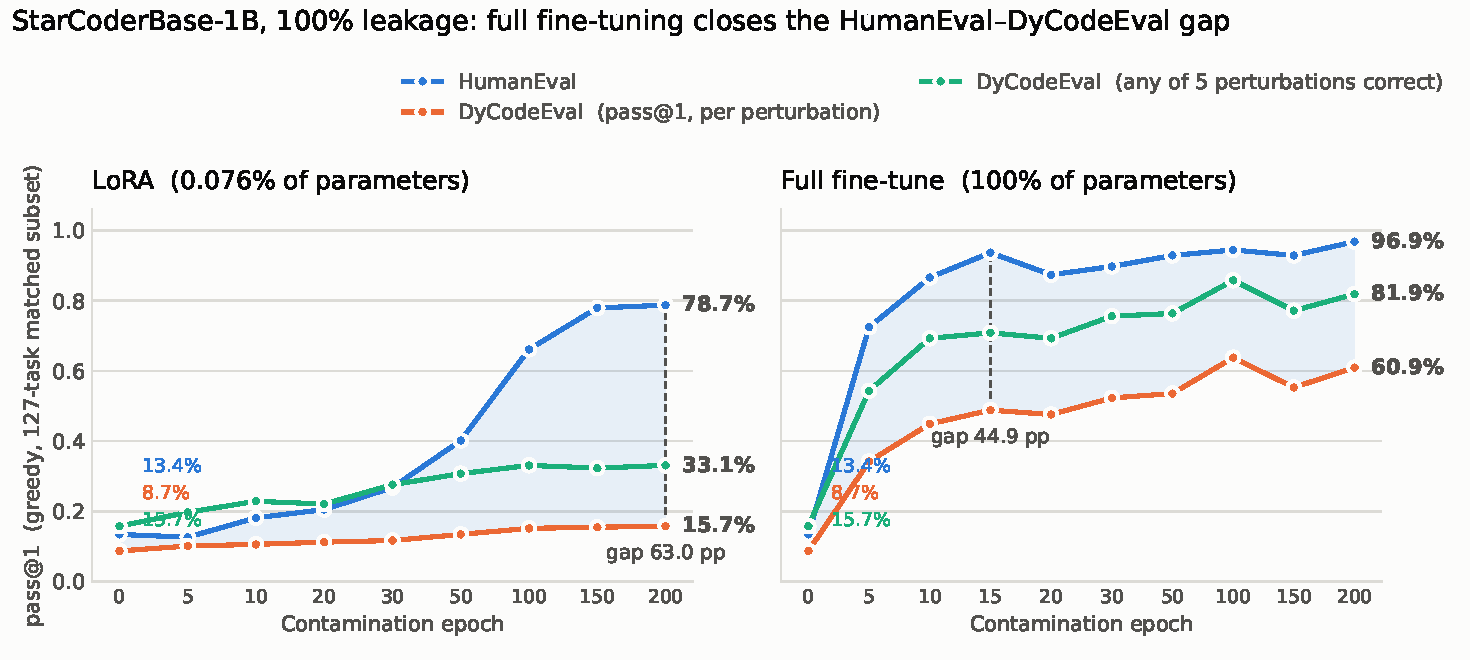
\includegraphics[width=\linewidth, trim=0 0 0 26, clip]{fig_peft_vs_full.pdf}
\vspace{-5mm}
\caption{Motivating example: StarCoderBase-1B, 100\% leakage (greedy pass@1, 127 tasks). Under LoRA, DyCodeEval stays flat and the rewrites seem to work. Under full fine-tuning, it climbs to 60.9\%, so many rewrites no longer block memorization.}
\label{fig:motiv}
\vspace{-3mm}
\end{figure}

\paragraph{Why it matters.} Our preliminary experiments show that the assumption often fails (Fig.~\ref{fig:motiv}). We contaminated StarCoderBase-1B~\cite{starcoder} with leaked HumanEval solutions. Under LoRA~\cite{lora}, which trains 0.076\% of the parameters, HumanEval rises to 78.7\% while DyCodeEval stays at 15.7\%, a 63.0\,pp gap that makes the rewrites look effective. Under full fine-tuning, the same rewrites break down: DyCodeEval pass@1 rises from 8.7\% to 60.9\%, and for 96 of 127 tasks at least one rewrite produces the canonical solution \emph{verbatim}, even though the model never saw any rewrite. Whether a perturbation works thus depends on the model and how it was contaminated.

\paragraph{Why it is challenging.} Leakiness varies \emph{within} a task. Among the 83 tasks that the contaminated model newly solved, 275 of 415 rewrites (66\%) recalled the solution verbatim, and 46 tasks had a mix of leaky and effective rewrites. Simple similarity also fails. In our earlier analysis, raw cosine similarity between prompt embeddings separated matched from unrelated prompts with AUROC of only 0.54, because decoder embeddings are highly anisotropic (matched and unrelated pairs differ by only 0.0035 in cosine).

\paragraph{Research question.} \emph{Can features from a model's prompt representations, and from how fine-tuning changes them, predict per rewrite whether memorized-solution recall survives the perturbation, and can they do so better than text-only baselines, reaching AUROC $\geq$ 0.75 on held-out tasks?}

%%%%%%%%%%%%%%%%%%%%%%%%%%%%%%%%%%%%%%%%%%%%%%%%%%%%%%%%%%%%%%%%%%%%%%%%%%
\section{Related Work and Research Gap}

\textbf{Dynamic benchmarks.} DyCodeEval~\cite{dycodeeval} rewrites HumanEval/MBPP problems into new scenarios with an LLM, and EvoEval~\cite{evoeval} evolves problems into new variants. Both validate their rewrites \emph{on average} and treat every variant as an equally valid probe. \textbf{Contamination detection.} Likelihood-based detectors such as Min-K\% Prob~\cite{mink} decide whether a \emph{model} saw a given text. \textbf{Gap.} No existing method evaluates whether an \emph{individual rewrite} still acts as a retrieval key for a memorized answer, and none predicts this per model. Our project fills this gap.

%%%%%%%%%%%%%%%%%%%%%%%%%%%%%%%%%%%%%%%%%%%%%%%%%%%%%%%%%%%%%%%%%%%%%%%%%%
\section{Proposed Method}


We treat perturbation quality as supervised binary classification over (model, task, rewrite) triples. \textbf{Labels} come from \emph{known} contamination. We fine-tune a model on leaked solutions and decode each rewrite greedily. A rewrite is labeled leaky if the edit similarity between the generated function body and $g_t$ (signature and docstring stripped) is at least $\tau{=}0.95$ and the base model did not reach $\tau$ on the same rewrite. Only tasks whose original prompt the contaminated model has memorized are included. \textbf{Features} use $h^\ell(x)$, the mean-pooled layer-$\ell$ hidden state over docstring tokens:
(F1) base-model cosine between $x_t$ and $x'_{t,k}$ at each layer, after mean-centering and whitening to remove anisotropy, and the rank of $x_t$ among all 164 originals when $x'_{t,k}$ is the query;
(F2) the fine-tuning shift $\Delta^\ell(x)=h^\ell_\theta(x)-h^\ell_{\theta_0}(x)$: alignment $\cos(\Delta^\ell(x_t),\Delta^\ell(x'_{t,k}))$, norm ratio, and the change in pair cosine;
(F3) surface overlap: prompt edit similarity, identifier overlap, and whether doctests are kept;
(F4) base-model likelihood gap $\log p(g_t\mid x')-\log p(g_t\mid x)$~\cite{mink}.
\textbf{Classifiers} are logistic regression, gradient-boosted trees, and a small MLP probe on $[u;v;|u{-}v|;u\odot v]$ with learned layer weights. \textbf{Pretrained models and adaptation.} StarCoderBase~\cite{starcoder} (1B, 15.5B) serves as the evaluated model family. Contamination is induced by full fine-tuning and by LoRA~\cite{lora}. MPNet and Qwen3-Embedding serve as frozen, model-agnostic text encoders. \textbf{Course topics} covered include representation learning, probing of pretrained models, full vs.\ parameter-efficient fine-tuning, supervised classification, and grouped cross-validation.

%%%%%%%%%%%%%%%%%%%%%%%%%%%%%%%%%%%%%%%%%%%%%%%%%%%%%%%%%%%%%%%%%%%%%%%%%%
\section{Dataset and Experiments}

\textbf{Data.} HumanEval~\cite{humaneval} has 164 Python problems with canonical solutions and tests. DyCodeEval~\cite{dycodeeval} provides 5 rewrites for each of 127 of these problems, 635 in total. Our contaminated checkpoints (already trained) are StarCoderBase-1B with full fine-tuning and LoRA, and 15.5B with LoRA, each at 25/50/75/100\% leakage and up to 10 epoch milestones. This gives on the order of $10^4$ labeled triples. Unleaked tasks at partial leakage serve as negative controls.
\textbf{Splits.} We use 5-fold GroupKFold \emph{by task}, so that rewrites of one problem never appear in both train and test.
\textbf{Metrics.} We report AUROC (primary), AUPRC, F1, and calibration error.
\textbf{Baselines.} The baselines are random guessing, a threshold on raw last-layer cosine, surface features only, and MPNet/Qwen3 text-encoder features.
\textbf{Principal comparisons.}
(E1) Correlation analysis: per-layer features vs.\ leakiness and pass/fail, using a mixed-effects model with a random effect per task.
(E2) Settings: \emph{audit} (base and contaminated weights, F1--F4) vs.\ \emph{prospective} (evaluated model only, F1, F3, F4) vs.\ \emph{text-only}.
(E3) Generalization: train on one condition and test on another, across epochs, leakage levels, full$\to$LoRA, and 1B$\to$15.5B.
(E4) Benchmark repair: keep only rewrites predicted to be effective, and measure the reduction in contamination inflation, pass@1(contaminated) $-$ pass@1(base), against random filtering of the same size.
\textbf{Ablations.} We remove each feature group, compare a single layer with all layers, compare whitening on/off, and sweep $\tau\in[0.8,1.0]$.

%%%%%%%%%%%%%%%%%%%%%%%%%%%%%%%%%%%%%%%%%%%%%%%%%%%%%%%%%%%%%%%%%%%%%%%%%%
\section{Novelty}

Prior work \emph{generates} perturbed problems~\cite{dycodeeval,evoeval} or detects contamination at the \emph{model} level~\cite{mink}. This project goes beyond reproducing either. It (i) shows under controlled, known contamination that many semantics-preserving rewrites still retrieve memorized solutions verbatim, with this varying across rewrites of the same problem and across fine-tuning regimes; (ii) learns the first \emph{per-rewrite, per-model} classifier of perturbation effectiveness from representation geometry and its fine-tuning shift; and (iii) uses the classifier to filter a dynamic benchmark, turning ``perturb and hope'' into ``perturb and verify.''

%%%%%%%%%%%%%%%%%%%%%%%%%%%%%%%%%%%%%%%%%%%%%%%%%%%%%%%%%%%%%%%%%%%%%%%%%%
\section{Feasibility and Fallback Plan}

\textbf{Data and compute.} All datasets are public, and all contaminated checkpoints, generations, and pass/fail results already exist. The remaining compute is feature extraction: forward passes over about 800 prompts per checkpoint, which takes minutes per 1B checkpoint on one GPU of the university cluster. The classifiers train on a CPU.
\textbf{Risks and fallbacks.}
(1) If embedding features are weak, we fall back to surface and likelihood features and report the negative result for geometry.
(2) If the labels are too imbalanced (e.g., under LoRA), we lower $\tau$ or regress the continuous edit similarity.
(3) If transfer across models fails, we train a per-model classifier, which is the stated goal.
(4) With only 127 independent tasks, overfitting is a risk, so we use regularized models, grouped splits, and bootstrap confidence intervals.

%%%%%%%%%%%%%%%%%%%%%%%%%%%%%%%%%%%%%%%%%%%%%%%%%%%%%%%%%%%%%%%%%%%%%%%%%%
\section{Timeline and Responsibilities}

\begin{itemize}\tightlist
\item \textbf{Wk 1--2:} per-layer feature extraction for all checkpoints; build the label table.
\item \textbf{Wk 3--4:} E1 correlation analysis; baselines.
\item \textbf{Wk 5--6:} E2 classifiers and ablations; \emph{milestone report}.
\item \textbf{Wk 7--8:} E3 generalization; E4 benchmark repair.
\item \textbf{Wk 9--10:} final analysis, figures, and \emph{final report}.
\end{itemize}
\textbf{Responsibilities.} \emph{Eshgin Hasanov:} contaminated checkpoints, feature extraction, and labeling. \emph{Osama Altarawneh:} classifiers, baselines, and ablations (E1, E2). \emph{Hongjie Tian:} generalization and benchmark-repair experiments (E3, E4). All members share the writing of the milestone and final reports.

{\small
\bibliographystyle{ieeetr}
\bibliography{egbib}
}

\end{document}
